%!TEX root = Slic3r-Manual.tex

\section{Vitesse} % (fold)
\label{sec:speed}
\index{speed}
\index{vitesse}

Une fois que l'imprimante produit de mani\`ere fiable des impressions de bonne qualit\'e, il peut \^etre souhaitable d'augmenter la vitesse. Faire cela offre plusieurs avantages, le plus \'evident est que les r\'esultats sont produits plus rapidement, mais aussi que le temps d'impression plus court peuvent \^etre utilis\'es dans la production de plus de couches, pour la m\^eme hauteur de couche, am\'eliorant ainsi la qualit\'e d'impression perçue. Un avantage suppl\'ementaire est qu'un mouvement plus rapide de d\'eplacement entre les extrusions, peut r\'eduire les effets de suintement.

La meilleure approche consiste \`a incr\'ementer les diff\'erents param\`etres de vitesses par petites \'etapes et observer l'effet de chaque changement a sur la qualit\'e d'impression. La vitesse de d\'eplacement (travel speed) est un point de d\'epart sur, et il n'est pas irr\'ealiste d'atteindre des vitesses allant jusqu'\`a 250mm/s (si votre imprimante peut le g\'erer). Les r\'eglages de la vitesse de p\'erim\`etres (p\'erimeters), de remplissage (infill) sont disponible en mode simple, et la r\`egle g\'en\'erale est que le p\'erim\`etre aille plus lentement que le remplissage afin de r\'eduire les imperfections \'eventuelles sur la surface (remplissage peut \^etre plus rapide parce que de l\'egers d\'efauts ne seront que importants).

Le Mode Expert offre plus de param\`etres pour r\'egler finement la vitesse de l'imprimante. La diff\'erenciation entre les p\'erim\`etres ext\'erieurs (external), petits (small) et d'autres p\'erim\`etres, remplissage (infill), et les ponts (bridge)et les vide (gap) sont disponibles, ainsi que la capacit\'e de ralentir la premi\`ere couche.

\begin{figure}[H]
\centering
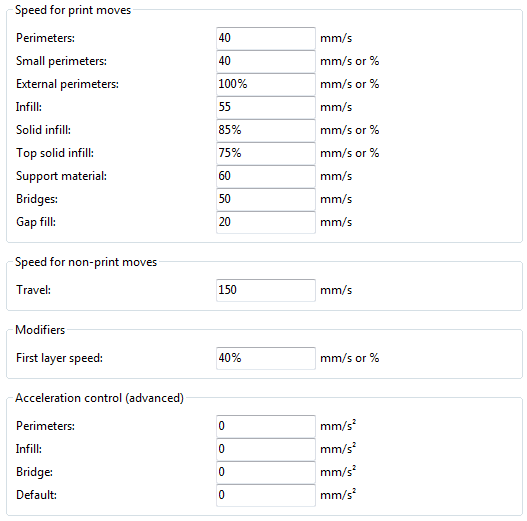
\includegraphics[keepaspectratio=true,width=1\textwidth]{expertmode/speed_advanced_settings.png}
\caption{Param\`etres de vitesse en mode expert.}
\label{fig:speed_advanced_settings}
\end{figure}


Le cas \'ech\'eant, une valeur peut \^etre donn\'ee en pourcentage. C'est par rapport \`a la valeur pr\'ec\'edente, par exemple 50\% de remplissage solide sera la moiti\'e de la valeur d\'efinie pour le remplissage.
\index{Print Settings!Speed}
\index{Param\`etres d'Impression!Vitesse}
\index{Print Settings!Speed!Perimeters}
\index{Param\`etres d'Impression!Vitesse!P\'erim\`etres}
\index{Print Settings!Speed!Small perimeters}
\index{Param\`etres d'Impression!Vitesse!P\'erim\`etres courts}
\index{Print Settings!Speed!External perimeters}
\index{Param\`etres d'Impression!Vitesse!P\'erim\`etres externes}
\index{Print Settings!Speed!Infill}
\index{Param\`etres d'Impression!Vitesse!Remplissage}
\index{Print Settings!Speed!Solid infill}
\index{Param\`etres d'Impression!Vitesse!Remplissage plein}
\index{Print Settings!Speed!Top solid }
\index{Param\`etres d'Impression!Vitesse!Haut plein}
\index{Print Settings!Speed!Support material}
\index{Param\`etres d'Impression!Vitesse!Support}
\index{Print Settings!Speed!Bridges}
\index{Param\`etres d'Impression!Vitesse!Pont}
\index{Print Settings!Speed!Gap fill}
\index{Param\`etres d'Impression!Vitesse!Remplissage des trous}
\index{Print Settings!Speed!Travel}
\index{Param\`etres d'Impression!Vitesse!D\'eplacement}
\index{Print Settings!Speed!First layer speed}
\index{Param\`etres d'Impression!Vitesse!Vitesse de la premi\`ere couche}

Quelques directives g\'en\'erales pour chaque option:
\begin{itemize}
	\item \texttt{Perimeters} (p\'erim\`etres) - En mode expert ce param\`etre peut \^etre l\'eg\`erement supp\'erieur que le param\`etre \texttt{External perimeters} (p\'erim\`etres externes), peut \^etre utilis\'e pour assurer les faces externes sans d\'efaut.
	\item \texttt{Small perimeters} (petits p\'erim\`etres) - Conçu pour les trous, les \^iles et les d\'etails fins, une vitesse plus lente ici est recommand\'ee.
	\item \texttt{External perimeters} (p\'erim\`etres externes) - Une valeur l\'eg\`erement plus lente peut assurer des surfaces propres.
	\item \texttt{Infill} (remplissage) - Aussi vite que vous le pouvez sans compromettre l'int\'egrit\'e de la structure de remplissage. Les extrusions rapides peuvent se briser et entra\^iner des points faibles.
	\item \texttt{Solid infill} (remplissage solid) - L'extrusion pour le fond du mod\`ele, et les couches solides suppl\'ementaires est g\'en\'eralement un peu plus lente que le pour remplissage mais plus rapide que pour les p\'erim\`etres.
	\item \texttt{Top solid infill} (remplissage solid du dessus) - Pr\'evoyez du temps pour que l'extrusion couvre proprement les couches sup\'erieures pr\'ec\'edentes qu'elle aboutisse \`a une surface sup\'erieure soign\'e. les derni\`eres couches doivent parfaitement combl\'ees la structure de remplissage, pr\'eparer la voie \`a une finition soign\'ee.
	\item \texttt{Support material} (support) - G\'en\'eralement les structures d'appui sont rapide et sale, et tant que que la base est correctement support\'ee, ils peuvent \^etre construits aussi rapidement que possible.
	\item \texttt{Bridges} (ponts) - Obtenir une distance d'extrusion de port\'ee d\'epend de la mati\`ere et du refroidissement. Aller trop lentement se traduira par l'affaissement, trop rapidement entra\^inera des brins cass\'es. L'exp\'erimentation est ici la cl\'e, mais g\'en\'eralement les pontages se r\'ealise plus lentement que les p\'erim\`etres.
	\item \texttt{Gap fill} (remplissage des vides) - Le remplissage de petits vides engendre de rapide oscillations de l'extrudeuse, la r\'esultante des tremblements et r\'esonance pourrait avoir un effet n\'efaste sur l'imprimante. Une valeur inf\'erieure peut ici s'en pr\'emunir cela. Un r\'eglage \`a z\'ero d\'esactive le remplissage de vide compl\`etement.
	\item \texttt{Travel} (d\'eplacement) - Aussi rapidement que votre imprimante permette afin de minimiser les suintements.
	\item \texttt{First layer speed} (vitesse de la 1ere couche) - Comme mentionn\'e dans la section \ref{sec:the_important_first_layer}, fixer correctement la prem\`ere couche est important, et un rythme plus lent aide \'enorm\'ement. D\'efinir un valeur de 50\%, voire moins, peut vraiment aider.
\end{itemize}

\index{Print Settings!Speed!Acceleration control}
\index{Param\`etres d'Impression!Vitesse!Crontrole de l'acc\'el\'eration}
\texttt{Acceleration control} est un param\`etre avanc\'e permettant les param\`etres d'acc\'el\'eration pour les p\'erim\`etres, remplissage, pont, ainsi que d'un r\'eglage par d\'efaut, \`a faire. D\'ecider quelles valeurs r\'egler d\'epend des capacit\'es de la machine. Tous les param\`etres dans le firmware peuvent \^etre un bon point de d\'epart.

Tenir compte des restrictions impos\'ees par le firmware comme beaucoup ont des param\`etres de vitesse de s\'ecurit\'e maximale pour chaque axe.

% section speed (end)